\documentclass[sigconf,nonacm]{acmart}

%% Remove ACM copyright box
\setcopyright{none}
\settopmatter{printacmref=false}
\renewcommand\footnotetextcopyrightpermission[1]{}

%% Packages
\usepackage{booktabs}
\usepackage{tabularx}
\usepackage{tikz}
\usepackage{pgfplots}
\pgfplotsset{compat=1.18}
\usetikzlibrary{shapes.geometric, arrows.meta, positioning, fit, backgrounds, calc}
\usepackage{xcolor}
\usepackage{microtype}
\usepackage{enumitem}
\usepackage{multirow}

%% Define custom colors
\definecolor{reconcolor}{HTML}{2C3E50}
\definecolor{weapcolor}{HTML}{1A5276}
\definecolor{delivcolor}{HTML}{117A65}
\definecolor{exploitcolor}{HTML}{7D6608}
\definecolor{c2color}{HTML}{6E2F8A}
\definecolor{actioncolor}{HTML}{922B21}
\definecolor{lightgray}{HTML}{F2F3F4}
\definecolor{accentblue}{HTML}{2471A3}

%%
%% Document metadata
%%
\title{Aligning Threat Actor TTPs to the Cyber Kill Chain:\\
Anticipating Future Cyber Threats with the MITRE ATT\&CK Framework}

\author{Ezekiel Ologunde}
\affiliation{%
  \institution{Independent Researcher}
  \country{United States}
}
\email{ezekiel.ologunde@example.com}

\date{October 2025}

%%
%% Abstract
%%
\begin{abstract}
This paper explores how the MITRE ATT\&CK Framework can be leveraged to anticipate
the evolution of threat actor tactics, techniques, and procedures (TTPs) within the
context of the Cyber Kill Chain. Drawing from insights presented at the 16th Annual
Billington Cybersecurity Summit, this paper connects academic and practical cybersecurity
perspectives, focusing on architectural resilience, data protection, and strategic planning.
The discussion examines how organizations can translate intelligence about TTPs into
stronger cybersecurity architectures and adaptive defenses against emerging technologies
such as artificial intelligence (AI) and quantum computing. By fusing predictive analytics
with ATT\&CK datasets, defenders can shift from reactive postures to anticipatory
resilience---securing not only data, but the trust and stability of entire digital ecosystems.
\end{abstract}

\keywords{MITRE ATT\&CK, Cyber Kill Chain, Threat Intelligence, Cybersecurity
Architecture, TTPs, Zero Trust, AI Threats, Quantum Computing}

\begin{document}

\maketitle

%%
%% 1. Introduction
%%
\section{Introduction}

The cybersecurity landscape is evolving at an unprecedented rate. As highlighted
during the 16th Annual Billington Cybersecurity Summit (2025), the convergence of
artificial intelligence (AI), quantum computing, and automation is reshaping both
offensive and defensive cyber operations. Adversaries are increasingly leveraging AI for
reconnaissance, automated vulnerability discovery, and model manipulation. In this
complex environment, frameworks like MITRE ATT\&CK and the Cyber Kill Chain
provide structured methods for understanding, predicting, and countering threat actor
behavior~\cite{mitre2025}.

Traditional perimeter-based defenses are no longer sufficient against modern adversaries
who operate with precision, persistence, and adaptability. Security teams require
structured, intelligence-driven approaches that enable them to contextualize observed
behaviors, forecast future attack patterns, and architect layered defenses accordingly.
The convergence of two widely adopted frameworks---the Cyber Kill Chain and
MITRE ATT\&CK---offers exactly this capability.

The purpose of this paper is to demonstrate how organizations can align the MITRE
ATT\&CK framework with the Cyber Kill Chain to: (1) anticipate future TTP
evolution; (2) enhance architectural resilience; and (3) make informed cybersecurity
design decisions in the face of emerging threats. The remainder of the paper is
organized as follows. Section~\ref{sec:anticipate} examines how ATT\&CK supports
predictive threat modeling. Section~\ref{sec:alignment} details the stage-by-stage
alignment between ATT\&CK and the Cyber Kill Chain. Section~\ref{sec:architecture}
translates these insights into actionable architecture principles. Section~\ref{sec:future}
looks ahead at evolving threats in cyber-physical domains. Section~\ref{sec:conclusion}
concludes the paper.

%%
%% 2. Using MITRE ATT&CK to Anticipate Future TTP Evolution
%%
\section{Using the MITRE ATT\&CK Framework to Anticipate Future TTP Evolution}
\label{sec:anticipate}

The MITRE ATT\&CK framework is a globally recognized knowledge base that catalogs
adversary behavior across the entire cyberattack lifecycle~\cite{mitre2025}. By mapping
known TTPs, organizations can identify emerging attack patterns and forecast potential
adaptations. According to Thakur~\cite{thakur2025}, threat actors will increasingly
target AI models and machine learning systems themselves, marking a fundamental shift
from traditional endpoint or network-based attacks toward \emph{AI ecosystem exploitation}.

\subsection{Predictive Alignment}

Organizations can use ATT\&CK matrices to monitor how techniques evolve over time.
For instance, AI-assisted phishing (T1566) or AI-enabled reconnaissance (T1595) are
rapidly emerging as candidate sub-techniques within the framework. Predictive analytics
combined with ATT\&CK datasets can reveal correlations between adversary campaigns,
helping defenders preemptively adjust controls. This predictive alignment transforms
cybersecurity from a reactive discipline into a proactive one---enabling security teams
to anticipate attacker moves rather than simply respond to them.

\subsection{From Observation to Forecast}

The power of ATT\&CK lies not only in cataloging what adversaries have done, but
in surfacing \emph{what they are likely to do next}. By aggregating technique usage data
across threat groups, analysts can identify technique clusters that frequently co-occur,
revealing likely attack paths. When combined with threat intelligence feeds and behavioral
baselines, this supports the construction of predictive threat models that inform both
detection engineering and security architecture decisions.

%%
%% Kill Chain / ATT&CK Alignment Diagram (TikZ)
%%
\begin{figure*}[t]
\centering
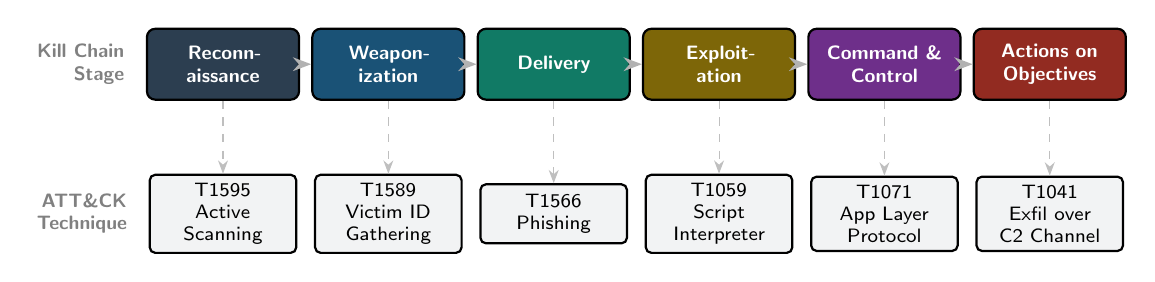
\begin{tikzpicture}[
  font=\small\sffamily,
  >=Stealth,
  stage/.style={
    rectangle, rounded corners=3pt,
    minimum width=1.72cm, minimum height=0.9cm,
    text centered, text width=1.65cm,
    inner sep=4pt, draw, thick,
    font=\scriptsize\sffamily\bfseries, text=white
  },
  techbox/.style={
    rectangle, rounded corners=2pt,
    minimum width=1.72cm, minimum height=0.75cm,
    text centered, text width=1.65cm,
    inner sep=3pt, draw, thick,
    fill=lightgray,
    font=\scriptsize\sffamily
  },
  arrow/.style={->, thick, gray!60}
]

%% --- Kill Chain stage nodes ---
\node[stage, fill=reconcolor]  (n1) at (0,0)     {Reconn-\\aissance};
\node[stage, fill=weapcolor]   (n2) at (2.1,0)   {Weapon-\\ization};
\node[stage, fill=delivcolor]  (n3) at (4.2,0)   {Delivery};
\node[stage, fill=exploitcolor](n4) at (6.3,0)   {Exploit-\\ation};
\node[stage, fill=c2color]     (n5) at (8.4,0)   {Command \&\\Control};
\node[stage, fill=actioncolor] (n6) at (10.5,0)  {Actions on\\Objectives};

%% --- Arrows between stages ---
\draw[arrow] (n1.east) -- (n2.west);
\draw[arrow] (n2.east) -- (n3.west);
\draw[arrow] (n3.east) -- (n4.west);
\draw[arrow] (n4.east) -- (n5.west);
\draw[arrow] (n5.east) -- (n6.west);

%% --- ATT&CK technique boxes below ---
\node[techbox] (t1) at (0,-1.9)   {T1595\\Active\\Scanning};
\node[techbox] (t2) at (2.1,-1.9) {T1589\\Victim ID\\Gathering};
\node[techbox] (t3) at (4.2,-1.9) {T1566\\Phishing};
\node[techbox] (t4) at (6.3,-1.9) {T1059\\Script\\Interpreter};
\node[techbox] (t5) at (8.4,-1.9) {T1071\\App Layer\\Protocol};
\node[techbox] (t6) at (10.5,-1.9){T1041\\Exfil over\\C2 Channel};

%% --- Connectors from stage to technique ---
\draw[dashed, gray!50, ->] (n1.south) -- (t1.north);
\draw[dashed, gray!50, ->] (n2.south) -- (t2.north);
\draw[dashed, gray!50, ->] (n3.south) -- (t3.north);
\draw[dashed, gray!50, ->] (n4.south) -- (t4.north);
\draw[dashed, gray!50, ->] (n5.south) -- (t5.north);
\draw[dashed, gray!50, ->] (n6.south) -- (t6.north);

%% --- Row labels ---
\node[font=\scriptsize\sffamily\bfseries, text=gray, left=0.15cm of n1, align=right]
  {Kill Chain\\Stage};
\node[font=\scriptsize\sffamily\bfseries, text=gray, left=0.15cm of t1, align=right]
  {ATT\&CK\\Technique};

\end{tikzpicture}
\caption{Alignment of MITRE ATT\&CK techniques with the Cyber Kill Chain phases.
  Dashed connectors link each kill chain stage to its representative ATT\&CK
  technique identifier. Color coding distinguishes stages by operational phase.}
\label{fig:killchain}
\end{figure*}

%%
%% 3. Aligning ATT&CK with the Kill Chain
%%
\section{Aligning MITRE ATT\&CK with the Cyber Kill Chain}
\label{sec:alignment}

The Cyber Kill Chain, developed by Lockheed Martin~\cite{lockheed2011}, outlines
seven sequential stages of a cyberattack: Reconnaissance, Weaponization, Delivery,
Exploitation, Installation, Command \& Control~(C2), and Actions on Objectives.
The MITRE ATT\&CK framework complements this model by detailing the specific
methods adversaries employ at each stage.

Figure~\ref{fig:killchain} illustrates this alignment visually. Table~\ref{tab:mapping}
provides a structured mapping of representative ATT\&CK techniques to each kill
chain phase, including the associated tactic category. This mapping enables security
teams to contextualize adversary behavior, track evolving technique patterns, and
reinforce defenses at each phase of the attack lifecycle.

By using this alignment, security architects can visualize how adversary operations
unfold and identify where their defensive layers are weakest. This is critical for
modern infrastructure, where threats are multi-vector and persistent.

\begin{table}[h]
\centering
\caption{Mapping ATT\&CK Techniques to the Cyber Kill Chain}
\label{tab:mapping}
\small
\begin{tabularx}{\columnwidth}{@{}l l X@{}}
\toprule
\textbf{Kill Chain Stage} & \textbf{ATT\&CK ID} & \textbf{Technique / Tactic} \\
\midrule
Reconnaissance      & T1595 & Active Scanning \newline \textit{Reconnaissance} \\
\addlinespace[3pt]
Weaponization       & T1589 & Gather Victim Identity Info \newline \textit{Resource Development} \\
\addlinespace[3pt]
Delivery            & T1566 & Phishing \newline \textit{Initial Access} \\
\addlinespace[3pt]
Exploitation        & T1059 & Command \& Scripting Interpreter \newline \textit{Execution} \\
\addlinespace[3pt]
Command \& Control  & T1071 & Application Layer Protocol \newline \textit{Command \& Control} \\
\addlinespace[3pt]
Actions on Objectives & T1041 & Exfiltration over C2 Channel \newline \textit{Exfiltration} \\
\bottomrule
\end{tabularx}
\end{table}

\subsection{Stage-by-Stage Analysis}

\textbf{Reconnaissance (T1595).}
Threat actors begin by actively scanning targets to gather information about exposed
services, open ports, and system configurations. AI-augmented scanning tools can
dramatically accelerate this phase, increasing the volume and precision of data collected
before an attack is launched.

\textbf{Weaponization (T1589).}
During weaponization, adversaries collect victim identity information to craft
highly targeted payloads. The aggregation of personally identifiable information
from open-source intelligence (OSINT) sources has made spear-phishing campaigns
significantly more convincing.

\textbf{Delivery (T1566).}
Phishing remains the predominant delivery mechanism, and AI-generated content
is making lures increasingly difficult to detect. Future sub-techniques may formally
catalog AI-assisted phishing as a distinct variant within the ATT\&CK matrix.

\textbf{Exploitation (T1059).}
Command and scripting interpreters are exploited to execute malicious code post-delivery.
Living-off-the-land (LotL) techniques that abuse legitimate system binaries continue
to evade signature-based detection at this stage.

\textbf{Command \& Control (T1071).}
Adversaries leverage standard application layer protocols---HTTP, HTTPS, DNS---to
blend C2 traffic with legitimate network communication, complicating detection through
conventional traffic analysis.

\textbf{Actions on Objectives (T1041).}
The final phase involves achieving the adversary's goal, most commonly data exfiltration
over established C2 channels. Ransomware operators increasingly combine exfiltration
with encryption, applying a double-extortion model to maximize leverage.

%%
%% 4. Applying Framework Insights to Architecture
%%
\section{Applying Framework Insights to Cybersecurity Architecture}
\label{sec:architecture}

Translating ATT\&CK and Kill Chain insights into architectural decisions requires
integrating threat intelligence into both the design and operational layers of an
organization's security program. As Kolobashkin~\cite{kolobashkin2025} noted, adversaries
now actively exploit AI systems themselves, compelling architects to embed AI model
integrity validation directly into their security designs. Similarly, if threat intelligence
signals an increase in credential access attacks (T1110), architects should prioritize
zero-trust authentication and behavioral analytics at the access layer.

Cybersecurity architecture must therefore evolve from static defense perimeters to
\emph{adaptive, layered systems} that respond continuously to threat intelligence.
Three core architectural principles emerge from this analysis.

\subsection{Dynamic Defense Posture}

Integrating real-time ATT\&CK technique mapping into Security Information and
Event Management (SIEM) tooling allows analysts to correlate observed events with
known adversary behaviors. This reduces mean time to detect (MTTD) and enables
context-aware response playbooks that are anchored to specific kill chain stages rather
than generic alert categories.

\subsection{Zero Trust Design}

Many C2 and lateral movement techniques exploit implicit trust within internal
network zones. A zero-trust architecture---grounded in the principle of
\emph{never trust, always verify}---reduces the attack surface available to adversaries
who have already achieved initial access. Micro-segmentation, identity-centric access
controls, and continuous session validation are key implementation pillars.

\subsection{Resilient Infrastructure}

Deploying redundancy, immutable backups, and automated recovery strategies mitigates
the impact of Actions on Objectives phase techniques such as data exfiltration and
ransomware deployment. Resilience planning must account for both cyber and physical
disruption vectors, particularly for organizations operating critical infrastructure.

%%
%% Architecture Diagram (TikZ)
%%
\begin{figure}[h]
\centering
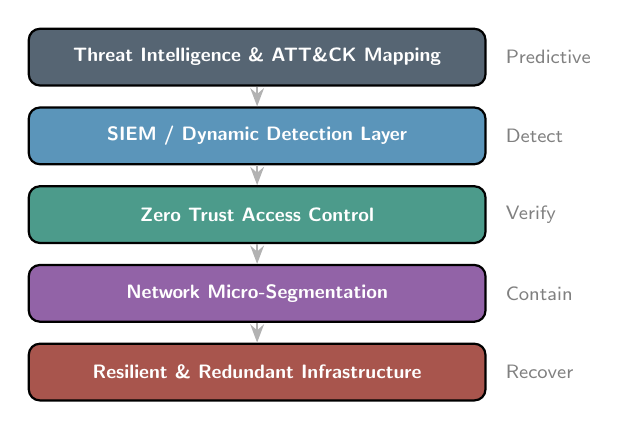
\begin{tikzpicture}[
  font=\scriptsize\sffamily,
  >=Stealth,
  layer/.style={
    rectangle, rounded corners=4pt,
    minimum width=5.8cm, minimum height=0.72cm,
    text centered, draw, thick,
    font=\scriptsize\sffamily\bfseries
  },
  label/.style={font=\scriptsize\sffamily, text=gray, align=left}
]

\node[layer, fill=reconcolor!80, text=white]  (l1) at (0, 3.2)
  {Threat Intelligence \& ATT\&CK Mapping};

\node[layer, fill=accentblue!75, text=white]  (l2) at (0, 2.2)
  {SIEM / Dynamic Detection Layer};

\node[layer, fill=delivcolor!75, text=white]  (l3) at (0, 1.2)
  {Zero Trust Access Control};

\node[layer, fill=c2color!75, text=white]     (l4) at (0, 0.2)
  {Network Micro-Segmentation};

\node[layer, fill=actioncolor!80, text=white] (l5) at (0,-0.8)
  {Resilient \& Redundant Infrastructure};

\draw[->, thick, gray!60] (l1.south) -- (l2.north);
\draw[->, thick, gray!60] (l2.south) -- (l3.north);
\draw[->, thick, gray!60] (l3.south) -- (l4.north);
\draw[->, thick, gray!60] (l4.south) -- (l5.north);

\node[label, right=0.12cm of l1] {Predictive};
\node[label, right=0.12cm of l2] {Detect};
\node[label, right=0.12cm of l3] {Verify};
\node[label, right=0.12cm of l4] {Contain};
\node[label, right=0.12cm of l5] {Recover};

\end{tikzpicture}
\caption{Intelligence-driven adaptive security architecture. Each layer maps to a
  defensive function derived from ATT\&CK and Kill Chain analysis.}
\label{fig:architecture}
\end{figure}

Figure~\ref{fig:architecture} illustrates how these layers compose an intelligence-driven
security architecture. Each stratum corresponds to a defensive function directly informed
by ATT\&CK technique patterns: from predictive threat modeling at the top to resilient
recovery capabilities at the base.

%%
%% 5. Anticipating Evolving Threats
%%
\section{Anticipating Evolving Threats: A Future Perspective}
\label{sec:future}

The Billington Cybersecurity Summit panel underscored that future threats will
increasingly target interconnected digital-physical systems, including critical
infrastructure and military assets~\cite{kolobashkin2025,thakur2025}. Adversaries
may exploit Internet of Things (IoT) ecosystems and cyber-physical systems,
fundamentally blurring the line between cyberattacks and kinetic warfare.

\subsection{AI-Augmented Adversaries}

The integration of AI into offensive operations is already underway. Automated
reconnaissance, AI-generated social engineering content, and adaptive malware that
modifies its own behavior to evade detection represent the near-term threat horizon.
Defending against these capabilities requires AI-based detection models trained on
adversarial simulation data derived from ATT\&CK technique inventories.

\subsection{Quantum Computing Threats}

Quantum computing poses a long-term but structural threat to current cryptographic
foundations. Adversaries pursuing \emph{harvest now, decrypt later} strategies are
already collecting encrypted data in anticipation of quantum decryption capability.
Organizations must begin cryptographic agility planning---implementing post-quantum
cryptographic standards to future-proof sensitive data assets.

\subsection{Cyber-Physical Convergence}

The challenge for cybersecurity architects lies in creating systems capable of
detecting, isolating, and recovering from both cyber and physical disruptions.
Operational technology (OT) and industrial control systems (ICS) that were previously
air-gapped are increasingly networked, expanding the attack surface to include physical
consequences. ATT\&CK for ICS provides a dedicated matrix for this domain, enabling
the same predictive alignment methodology to be applied to critical infrastructure
environments.

In practical terms, preparedness means training defensive AI models on simulated
threat campaigns derived from ATT\&CK, and continuously updating those models
as new TTPs emerge globally. Red team exercises grounded in ATT\&CK emulation
plans provide high-fidelity validation of defensive postures against realistic adversary
behavior~\cite{army2025}.

%%
%% 6. Conclusion
%%
\section{Conclusion}
\label{sec:conclusion}

The MITRE ATT\&CK framework, when aligned with the Cyber Kill Chain, provides
a structured lens through which to view, anticipate, and counter the evolution of
threat actor behavior. As the cybersecurity landscape continues to intertwine with AI
and quantum innovations, the ability to predict and adapt architectural defenses becomes
indispensable. Organizations that fuse these frameworks into their security architectures
can move from reactive defense to \emph{anticipatory resilience}---securing not just data,
but the trust and stability of their digital ecosystems.

Three key takeaways emerge from this analysis. First, ATT\&CK's breadth and depth
make it uniquely suited for predictive threat modeling when combined with behavioral
analytics and threat intelligence feeds. Second, mapping ATT\&CK techniques to
Kill Chain stages enables architects to identify and address the weakest defensive layers
in their environments before adversaries exploit them. Third, the emergence of AI- and
quantum-enabled attack vectors demands that architectural adaptation be treated as a
continuous, intelligence-driven process rather than a periodic exercise.

Future work should explore quantitative methods for scoring architectural resilience
against mapped ATT\&CK technique clusters, as well as empirical studies of how
ATT\&CK-aligned SIEM configurations reduce mean time to detect and respond across
industry sectors.

%%
%% References
%%
\bibliographystyle{ACM-Reference-Format}
\begin{thebibliography}{9}

\bibitem{kolobashkin2025}
I.~Kolobashkin.
\newblock Remarks at the {16th Annual Billington Cybersecurity Summit}.
\newblock Security Service of Ukraine, September 2025.

\bibitem{lockheed2011}
Lockheed Martin.
\newblock Intelligence-driven computer network defense informed by analysis of
  adversary campaigns and intrusion kill chains.
\newblock Technical report, Lockheed Martin Corporation, 2011.

\bibitem{mitre2025}
{MITRE Corporation}.
\newblock {MITRE ATT\&CK Framework}, 2025.
\newblock \url{https://attack.mitre.org/}.

\bibitem{thakur2025}
V.~Thakur.
\newblock Emerging threats and {AI}-driven cybersecurity challenges.
\newblock Broadcom Presentation, Billington Summit, September 2025.

\bibitem{army2025}
{U.S. Department of the Army}.
\newblock Army continuous transformation: Cyber modernization strategy.
\newblock Technical report, U.S. Army Cyber Command, 2025.

\end{thebibliography}

\end{document}
